\documentclass[10pt,english]{beamer}
%\documentclass[english,handout]{beamer} % For handouts
\usetheme[progressbar=frametitle,block=fill]{metropolis} %numbering=none

%%% USEFUL PACKAGES
%\usepackage{showframe} % For debugging positioning
\usepackage{etex} % If too many packages
% Encoding and language
\usepackage[utf8]{inputenc}
\usepackage{babel}
\usepackage{amsmath, amssymb}
\usepackage{natbib}
%\usepackage{booktabs}
%\usepackage{algorithmic}
\usepackage{algorithm}
\usepackage{caption}
%\usepackage{animate} % Animations
\usepackage{bm} % Bold math
\usepackage{bbm}
%\usepackage{url}
%\usepackage{pifont}
%\usepackage{ulem} % Used for strikeouts \sout
%\usepackage{stackengine}
%\usepackage{enumitem}
%\setlist[description]{leftmargin=\parindent,labelindent=\parindent}
%\usepackage{colortbl} % Used for colored rows in tables


%%% GRAPHICS
\usepackage{graphicx}
\graphicspath{{./figs/}}


%%% COLORS
\setbeamercolor{background canvas}{bg=white}
\def\BlankFrame{
	\bgroup
	%\pdfpageheight 29.7cm
	\setbeamercolor{background canvas}{bg=}
	\begin{frame}[plain]
	\end{frame}
	%\makeatletter
	%\pdfpageheight \beamer@paperheight
	%\makeatother
	\egroup}

\usepackage{xcolor}
\definecolor{DarkGreen}{HTML}{00B200}
\definecolor{LightBlue}{HTML}{0090D9}
\definecolor{gold}{rgb}{.812,.710,.231}
% Text markup
%\setbeamercolor{alerted text}{fg=red}
\newcommand{\blue}[1]{\textcolor{blue}{#1}}
\newcommand{\red}[1]{\textcolor{red}{#1}}
\newcommand{\grey}[1]{\textcolor{gray}{#1}}
\newcommand{\orange}[1]{\textcolor{mLightBrown}{#1}}
\newcommand\myheading[1]{\textbf{#1}}
\newcommand\myemph[1]{\underline{\emph{#1}}}
\newcommand\textexample[1]{\textit{\textbf{#1}}}

%%% SPACING
\newcommand\vws[1][1]{\vspace{#1\baselineskip}} % vertical white space
%\newcommand\strt[1][1.5ex]{\rule[-.05\baselineskip]{0pt}{#1}} % strut
\newcommand\strt[2]{\rule[-#1ex]{0pt}{#2ex}} % strut
\newcommand\Hrule{\vspace{1ex} \hrule \vspace{1ex}} % Horisontal rule with some space after

%%% MISC
\newcommand\articleref[4]{\noindent\begin{minipage}[t]{0.04\textwidth}
		\vspace{0pt} 
		\pgfuseimage{beamericonarticle}
	\end{minipage}%
	\begin{minipage}[t]{0.96\textwidth}
		\vspace{0pt}
		#1. \textbf{#2.} \textit{#3}, #4.
	\end{minipage}}

%%% METROPOLIS THEME SPECIFIC
\makeatletter
\setlength{\metropolis@progressonsectionpage@linewidth}{1pt}
\makeatother
%\setbeamercolor{progress bar}{fg=red,bg=red!50}


%%% TEXTPOS
\usepackage[absolute,overlay]{textpos} % option showboxes is useful in draft mode
\setlength{\TPHorizModule}{\paperwidth}
\setlength{\TPVertModule}{\paperheight}
\textblockorigin{0pt}{10mm} % start everything at top-left, below gray 


%%% TIKZ/PGFPLOTS
\usepackage{tikz}
\usetikzlibrary{arrows,positioning,calc,shapes.geometric}
%\usetikzlibrary{arrows,calc,shapes.geometric,decorations.pathmorphing,backgrounds,positioning,fit,petri,decorations.pathreplacing}
%\usepackage{pgfplots}
%\pgfplotsset{compat = 1.3}


%%% BLOCKS AND BOXES
% Changing colors of blocks
%\setbeamercolor{block title alerted}{bg=UURed,fg=palette primary.fg}
%\setbeamercolor{block body alerted}{bg=UURed!15}
\setbeamercolor{block title alerted}{bg=mLightBrown,fg=palette primary.fg}
\setbeamercolor{block body alerted}{bg=mLightBrown!15}
%\setbeamercolor{block title example}{bg=UUGreen,fg=palette primary.fg}
%\setbeamercolor{block body example}{bg=UUGreen!10}
% \mybox is a rectangular box
\usepackage{boxedminipage}
\setlength\fboxrule{2pt}
\setlength\fboxsep{2\fboxsep}
\newcommand\mybox[3][\textwidth]{
  {\color{#2}
    \begin{boxedminipage}{#1}
      {\color{palette primary.bg} #3}
    \end{boxedminipage}}%
}   
\usepackage{tcolorbox}
\tcbset{arc=1mm,grow to left by=3mm,grow to right by=3mm,left=2mm}
%\newenvironment{redbox}{%
%	\begin{tcolorbox}[colback=UURed!15,colframe=UURed]}{%
%	\end{tcolorbox}}
%\newenvironment{greenbox}{%
%	\begin{tcolorbox}[colback=UUGreen!15,colframe=UUGreen]}{%
%	\end{tcolorbox}}
\newenvironment{redbox}{%
	\begin{tcolorbox}[colback=red!15,colframe=red]}{%
	\end{tcolorbox}}
\newenvironment{greenbox}{%
	\begin{tcolorbox}[colback=DarkGreen!15,colframe=DarkGreen]}{%
	\end{tcolorbox}}
\newenvironment{graybox}{%
	\begin{tcolorbox}[colback=mDarkTeal!5,colframe=mDarkTeal]}{%
	\end{tcolorbox}}
\newenvironment{orangebox}{%
\begin{tcolorbox}[colback=mLightBrown!15,colframe=mLightBrown]}{%
	\end{tcolorbox}}
\newenvironment{bwbox}{%
	\begin{tcolorbox}[colback=white,colframe=black]}{%
\end{tcolorbox}}
\newenvironment{bluebox}{%
	\begin{tcolorbox}[colback=LightBlue!15,colframe=LightBlue]}{%
\end{tcolorbox}}


%%%%%%%%% NEW MACROS

\newcommand\imp[1]{\alert{\textbf{#1}}}
\newcommand\bfit[1]{\textbf{\textit{#1}}}
\newcommand\good{\color{DarkGreen}{$\blacktriangle$}} % used in lists
\newcommand\bad{\color{red}{$\blacktriangledown$}} % used in lists


\RequirePackage{amsmath, amssymb}
\RequirePackage{bbm}
%\RequirePackage{newtxmath}


% Convenience macro for referring to data source
\newcommand\sourceurl[2]{\small \grey{Data from \href{#1}{#2}}}

% Abbreviations
\RequirePackage{xspace}
\newcommand\pdf{pdf\xspace}
\newcommand\ifft{iff\xspace}
\newcommand\ex{\textbf{ex)}\xspace}

% General time series notation
\newcommand\T{n}  % Length of time series
\newcommand\rtheta{{\red{\theta}}}  % Parameter (color coded)
\newcommand\rthetah{{\red{\widehat\theta}}}  % Estimate (color coded)

% Neural netowkrs
\newcommand\h{\mathbf{h}} % Hidden state variable
\newcommand\zz{\mathbf{z}} % Generic input (vector)

% For OLS/AR
\newcommand\noise{\varepsilon}  % This is the noise in AR, but should it be the same as measurement noise in SSM?
\newcommand\noisevar{\sigma^2_\noise}
\newcommand\noisevarhat{\widehat\sigma^2_\noise}
\newcommand\X{\Phi}
\newcommand\y{\mathbf{y}}
\newcommand\bphi{\bm\phi}

% State space models
\newcommand\z{\alpha}  % State vector, general SSM
\newcommand{\obsnoise}{\varepsilon}
\newcommand{\statenoise}{\eta}
\newcommand{\varobs}{\sigma^2_{\varepsilon}}
\newcommand{\varstate}{\sigma^2_{\eta}}
% For structural time series
\newcommand{\trendnoise}{\zeta}
\newcommand{\seasnoise}{\omega}
\newcommand{\vartrend}{\sigma^2_{\trendnoise}}
\newcommand{\varseas}{\sigma^2_{\seasnoise}}

%
\newcommand\FF{T}
\newcommand\GG{R}
\newcommand\HH{Z}
\newcommand{\covobs}{\sigma_\epsilon^2}
\newcommand{\covstate}{Q}
\newcommand\initmean{a_1}
\newcommand\initcov{P_1}
% Kalman filter
\newcommand{\zpart}[2]{\z_{#1}^{#2}}
\newcommand{\wgt}[2]{\omega_{#1}^{#2}}
\newcommand{\wgtsum}[1]{\Omega_{#1}}
\newcommand\zhat[2]{\hat\z_{#1|#2}}
\newcommand\Phat[2]{P_{#1|#2}}
\newcommand\zpred[1]{\zhat{#1}{#1-1}}
\newcommand\Ppred[1]{\Phat{#1}{#1-1}}
\newcommand\zfilt[1]{\zhat{#1}{#1}}
\newcommand\Pfilt[1]{\Phat{#1}{#1}}
\newcommand\ypred[1]{\hat y_{#1|#1-1}}
\newcommand\Spred[1]{F_{#1|#1-1}}
\newcommand\Spredinv[1]{\Spred{#1}^{-1}}
\newcommand\epshat[2]{\hat{\obsnoise}_{#1|#2}}
\newcommand\etahat[2]{\hat{\statenoise}_{#1|#2}}

\newcommand{\statefun}{T}
\newcommand{\obsfun}{Z}
\newcommand{\estfun}{h}

\newcommand{\qd}{q} %State density
\newcommand{\md}{g} %Measure density

\newcommand{\rmd}{\mathrm{d}}

% SMC
\newcommand{\Np}{N}           % Number of particles
\newcommand{\Mp}{M}           % Number of particles in backward simulation



%\RequirePackage{color}
%\newcommand{\flnote}[1]{{\color{red}\textbf{[#1]}}} % Used for notes in text - color red
%\newcommand\Hrule{\vspace{1ex} \hrule \vspace{1ex}} % Horisontal rule with some space after; This is moved to beamer preamble

%%%%%%%%%%%%%%%%%%%%%%%%%%%%%%%%%%%%%%%%%%%%%%%%%%%%%%%%%%%%%%%%%%%%%%%%%%%%%%%%
%                            COMMANDS IN TEXT                                  %
%%%%%%%%%%%%%%%%%%%%%%%%%%%%%%%%%%%%%%%%%%%%%%%%%%%%%%%%%%%%%%%%%%%%%%%%%%%%%%%%
\newcommand\numtext[2]{#1\textsuperscript{#2}}
\newcommand\thsnd[1]{\ensuremath{#1\thinspace000}}
\newcommand{\peqref}[1]{\eqref{#1} on page~\pageref{#1}} % Page referencing for equations: "(1) on page 1"

%%%%%%%%%%%%%%%%%%%%%%%%%%%%%%%%%%%%%%%%%%%%%%%%%%%%%%%%%%%%%%%%%%%%%%%%%%%%%%%%
%                            SPECIFIC MATH                                     %
%%%%%%%%%%%%%%%%%%%%%%%%%%%%%%%%%%%%%%%%%%%%%%%%%%%%%%%%%%%%%%%%%%%%%%%%%%%%%%%%
% Models etc.
%\newcommand{\T}{T}            % Number of samples in data record
\newcommand{\parspace}{\Theta}                                   % Parameter space
\newcommand{\parameter}{\theta}                                  % Parameter
% Spaces
\newcommand{\setX}{\ensuremath{\mathsf{X}}}                      % State-space X
\newcommand{\sigmaX}{\ensuremath{\mathcal{X}}}                   % Sigma algebra on X
\newcommand{\setY}{\ensuremath{\mathsf{Y}}}                      % State-space Y
\newcommand{\sigmaY}{\ensuremath{\mathcal{Y}}}                   % Sigma algebra on Y
\newcommand{\setZ}{\ensuremath{\mathsf{Z}}}                      % State-space Z
\newcommand{\sigmaZ}{\ensuremath{\mathcal{Z}}}                   % Sigma algebra on Z

%%%%%%%%%%%%%%%%%%%%%%%%%%%%%%%%%%%%%%%%%%%%%%%%%%%%%%%%%%%%%%%%%%%%%%%%%%%%%%%%
%                           GENERAL MATH                                       %
%%%%%%%%%%%%%%%%%%%%%%%%%%%%%%%%%%%%%%%%%%%%%%%%%%%%%%%%%%%%%%%%%%%%%%%%%%%%%%%%

% ======== Miscellaneous symbols ========
\newcommand\eqdef{:=}
\newcommand\defeq{=:}
\newcommand\const{\text{const.}}
%\newcommand\eqdef{\stackrel{\text{\scriptsize def}}{=}}

\newcommand\iid{iid}
\newcommand{\iidsim}{\stackrel{\text{\iid}}{\sim}} % iid simulation
\newcommand{\process}[1]{\{#1\}_{t\geq 1}}       % Process (time index t)
\newcommand{\range}[2]{#1, \, \dots, \, #2}      % Range = 1, ..., N
\newcommand{\crange}[2]{\{#1, \, \dots, \, #2\}} % Curly range = {1, ..., N}
\newcommand{\prange}[2]{(#1, \, \dots, \, #2)}   % Parenthesised range = (1, ..., N)
\newcommand{\bwdrange}[2]{#1 : -1 : #2}          % Range = N, ..., 1
\newcommand{\approxpropto}{\stackrel{\sim}\propto}

% Tight dots between \int and \int in a multidimensional integral
\newcommand{\tightcdots}{\hspace*{-0.38em}\cdot\hspace*{-0.3em}\cdot\hspace*{-0.3em}\cdot\hspace*{-0.38em}}

% Arrows - convergence and mappings
% \mapsto                                                     % Mappings, x \mapsto f(x)
\newcommand{\fromto}{\rightarrow}                             % Mapping from set A to set B; f: A \fromto B
\newcommand{\goesto}{\rightarrow}                             % limits used in n \goesto \infty
\newcommand{\goestosmall}{\to}                                % limits used in \lim_{n \goestosmall \infty}
\newcommand{\convP}{\stackrel{\probab}\longrightarrow}        % Convergence in probability
\newcommand{\convD}{\stackrel{\textrm{D}}\longrightarrow}     % Convergence in distribution

% ======== Standard spaces  ========
\newcommand{\naturals}{\ensuremath{\mathbb{N}}}               % Natural numbers
\newcommand{\reals}{\ensuremath{\mathbb{R}}}                  % Real numbers
\newcommand{\nonnegatives}{\reals_{\smaller +}}               % Nonnegative numbers
\newcommand{\positives}{\reals_{\smaller ++}}                 % Positive numbers
\newcommand{\nonnegativedefinites}[1]{S_{\smaller +}(#1)}     % Nonnegative #1 x #1 matrices
\newcommand{\positivedefinites}[1]{S_{++}(#1)}                % Positive #1 x #1 matrices

% ======== Matrices ========
\newcommand{\eye}[1]{I_{#1}}                     % Identity matrix
\newcommand{\+}{\mathsf{T}}                      % Transpose
\newcommand{\kronecker}{\raisebox{1pt}{\ensuremath{\otimes}}} % Kronecker product
\DeclareMathOperator*\diag{diag}
\DeclareMathOperator*\trace{tr}

% ======== Operators, calculus etc. ========
\newcommand{\Ordo}{O}                            % Big ordo
\newcommand{\supnorm}[1]{\|#1\|_\infty}          % Supremum norm
\newcommand\osc{\text{osc}}                      % Oscillator norm
\newcommand{\grad}{\nabla}                       % Gradient
\newcommand{\complementof}[1]{\ensuremath{#1^\mathsf{c}}} % Set complement
\renewcommand\vec{\text{vec}}
\DeclareMathOperator*\supp{supp}                          % Support
\DeclareMathOperator*\card{card}                          % Set cardinality
\DeclareMathOperator*\rank{rank}                          % Rank
\DeclareMathOperator*\sign{sign}                          % Signum function
\DeclareMathOperator*\argmax{arg\,max}
\DeclareMathOperator*\argmin{arg\,min}

% ======== Probability ========
\newcommand{\Prb}{\ensuremath{\mathbb{P}}}                       % Probability
\newcommand{\E}{\ensuremath{\mathbb{E}}}                         % Expectation
\newcommand{\var}{\ensuremath{\mathrm{Var}}}                     % Variance
\newcommand{\cov}{\ensuremath{\mathrm{Cov}}}                     % Covariance
\newcommand{\cor}{\ensuremath{\mathrm{Corr}}}                     % Correlation
\newcommand{\I}{\ensuremath{\mathbbm{1}}}						 % Indicator function

%\newcommand{\abscont}{\ensuremath{\ll}}          % Absolute continuity
\renewcommand\mid{\,\vert\,} % I don't really like that \mid produces rubber lengths. Sometimes, we get very large white spaces p(x    |   y), and it can produce line breaks after "p(x |" . Is the non-rubber definition here better?
\newcommand\Mid{\,\middle\vert\,} % Stretchable |, to use with \left \right - N.B. This produces a longer | in general. Does that look better than a standard \mid?


% Distributions
\newcommand{\N}{\ensuremath{\mathcal{N}}}        % Normal
\newcommand{\uni}{\ensuremath{\mathcal{U}}}      % Uniform
\newcommand\MN{\mathcal{MN}}                     % Matrix normal
\newcommand\IW{\mathcal{IW}}                     % Inverse-Wishart
\newcommand\GP{\mathcal{GP}}                     % Gaussian process
\DeclareMathOperator*\Mult{Mult}                 % Multinomial
\DeclareMathOperator*\cat{Cat}                   % Categorical
\DeclareMathOperator*\Discrete{Discrete}         % Categorical/alternative name
\DeclareMathOperator*\bin{Bin}                   % Binomial
\DeclareMathOperator*\gam{Gam}                   % Gamma
\DeclareMathOperator*\St{St}                     % Student's t
\DeclareMathOperator*\po{Po}                   % Binomial

%\usepackage{extendedalt}
%\usepackage{animate} % Animations
%\usepackage{../lindsten}
%\usepackage{movie15}
\usepackage{tikz}
\usepackage{listofitems} % for \readlist to create arrays

\hypersetup{
  colorlinks=true, urlcolor=blue, linkcolor=red
}

\title{732G12 Data Mining}
\subtitle{Föreläsning 3}
\date{}
\author{Josef Wilzén \\ IDA, Linköping University, Sweden}
\titlegraphic{\hfill
\includegraphics[height=1.2cm]{../LiU_primary_black.pdf}}
%\institute{Joint work with\dots}


%% MY DEF %%
\newcommand{\itm}[1]{\mathrm{Item}_{#1}}
\newcommand{\pausa}{\pause}
%\renewcommand{\pausa}{}
\tikzstyle{mynode}=[thick,draw=blue,fill=blue!20,circle,minimum size=22]


\newenvironment{nscenter}
 {\parskip=0pt\par\nopagebreak\centering}
 {\par\noindent\ignorespacesafterend}

\begin{document}

\maketitle

\begin{frame}{Dagens föreläsning}

    \begin{itemize}
        \item Linjära och icke-linjära modeller
        \item Splines
        \item GAM: Generalized additive model
    \end{itemize}
    
\end{frame}

\begin{frame}{Linjära och icke-linjära modeller}
    Inom både regression och klassificering har vi pratat om linjära modeller.

    Exempel:
    \begin{itemize}
        \item Linjär regression
        \item Linjär logistisk regression
    \end{itemize}

    Lätta att skatta och tolka $\rightarrow$ Kan inte lösa alla problem.
\end{frame}

\begin{frame}{Exempel klassificering}
   
   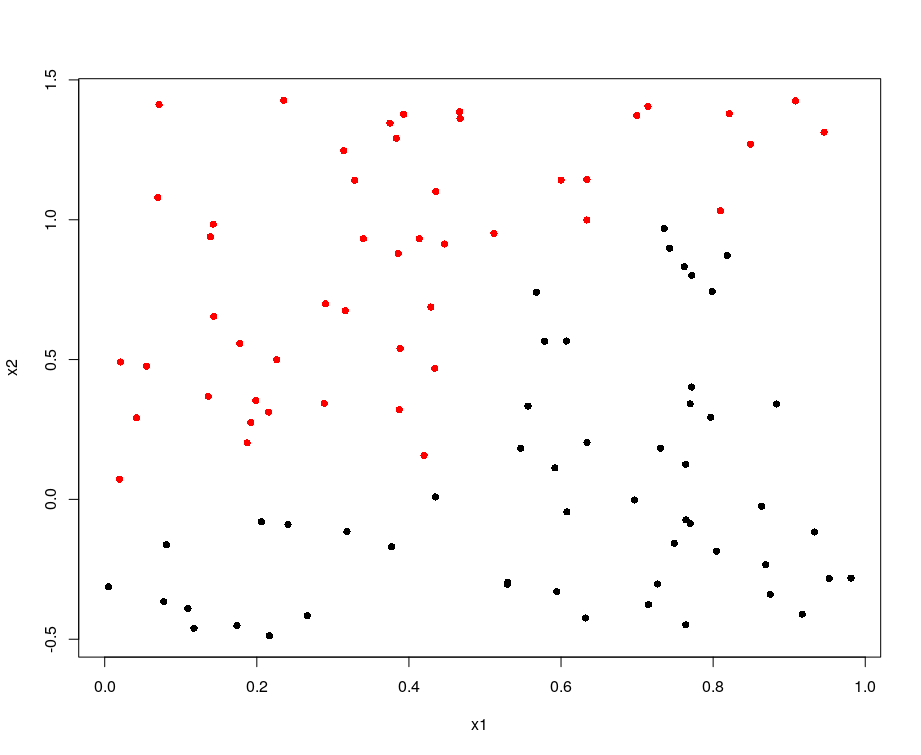
\includegraphics[scale=0.35]{non-linear_class_problem.png}
   
    100 observationer, två förklarande variabler, binär respons.

   
\end{frame}


\begin{frame}{Exempel - Klassificering}
    
    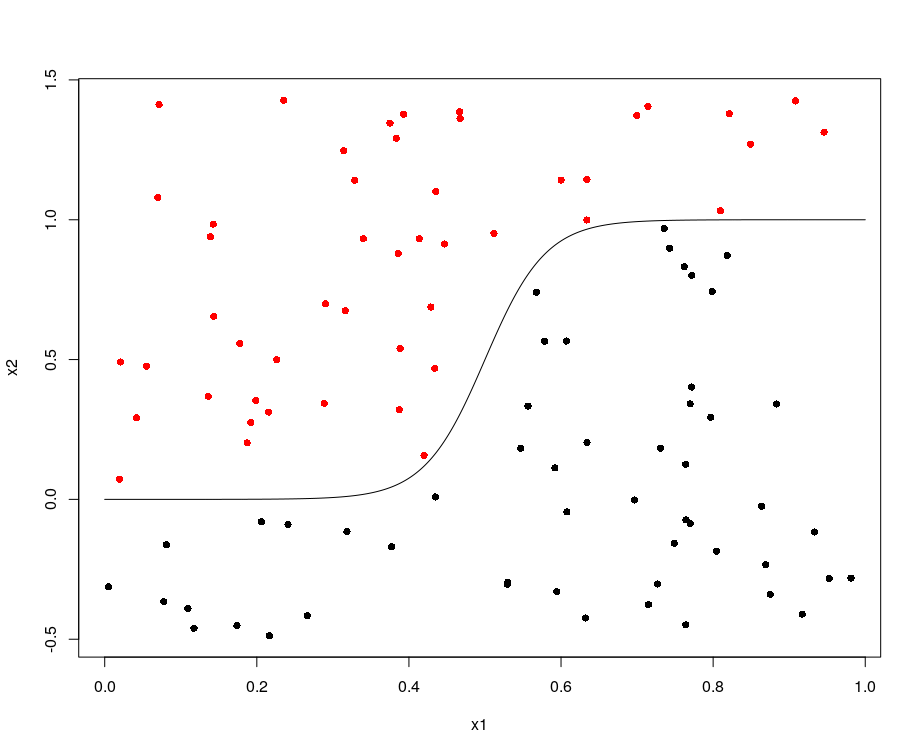
\includegraphics[scale=0.35]{non-linear class problem2.png}

    Sann beslutsregel: $x_2 \cdot (1 + \exp(-25 \cdot (x_1 - 0.5))) > 1$ $\qquad$ Bästa linjära?

\end{frame}



\begin{frame}{Icke-linjär regression}

    Vanlig linjär regression i en variabel:
    \begin{equation*}
        y_i = \beta_0 + \beta_1 x_i + \varepsilon_i, \qquad \varepsilon_i \sim \mathcal{N}(0, \sigma^2).
    \end{equation*}

    Vad gör vi om en linjär funktion inte passar till datan?

    \only<2>{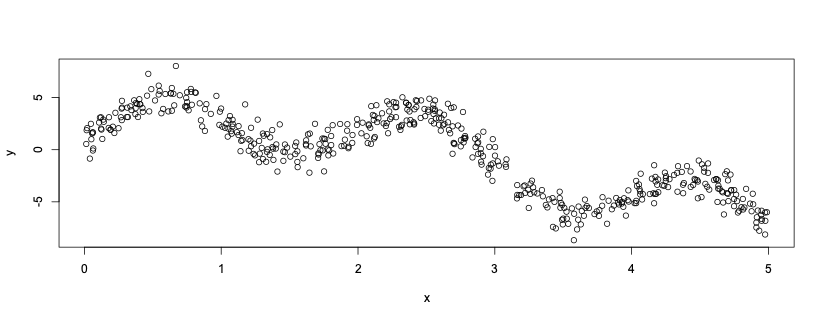
\includegraphics[width = \textwidth]{figs/nonLin.png}}
    \only<3>{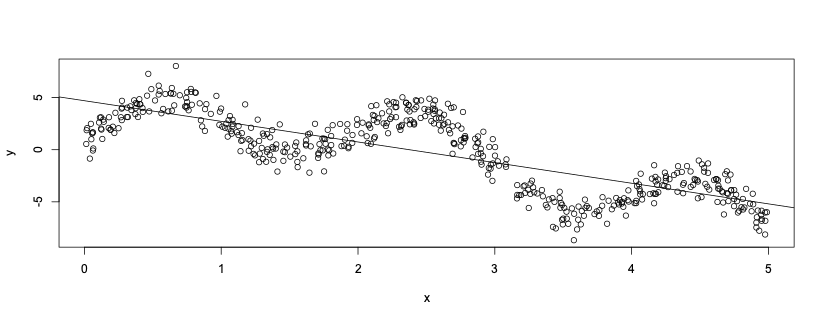
\includegraphics[width = \textwidth]{figs/nonLinWithLM.png}}
    
\end{frame}

\begin{frame}{Polynomregression}

    Ett alternativ är att modellera som ett polynom,
    \begin{equation*}
        y_i = \beta_0 + \beta_1 x_i + \beta_2 x_i^2 + \ldots + \beta_p x_i^p + \varepsilon_i.
    \end{equation*}

    Men vilken ordning $p$ ska vi ha?

    \only<2>{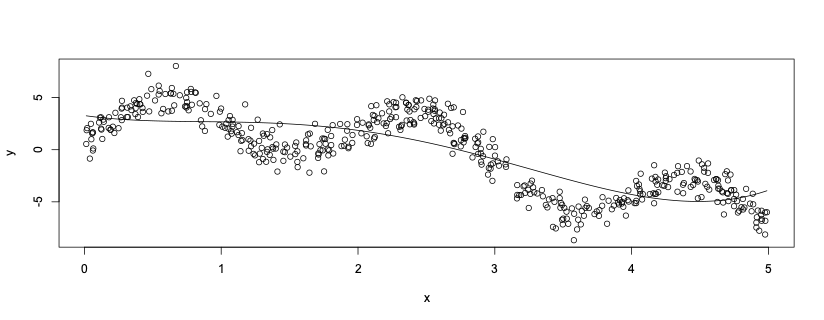
\includegraphics[width = \textwidth]{figs/nonLinWithPoly4.png}}
    \only<3>{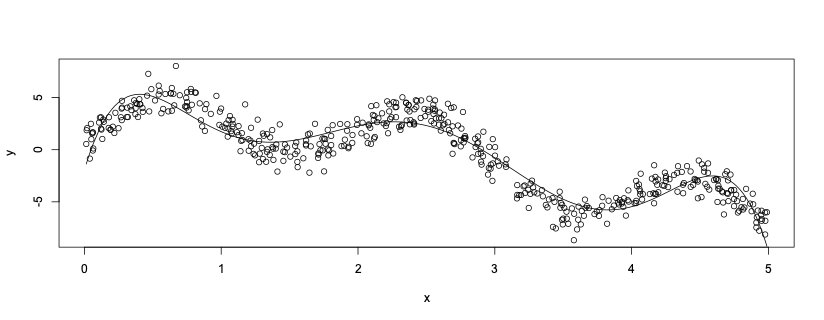
\includegraphics[width = \textwidth]{figs/nonLinWithPoly6.png}}
    \only<4>{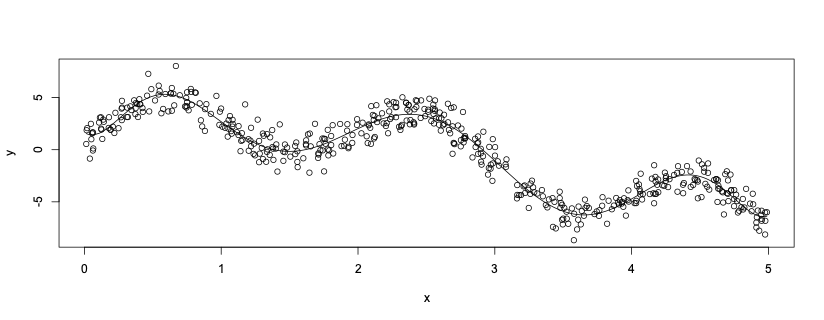
\includegraphics[width = \textwidth]{figs/nonLinWithPoly8.png}}
    
\end{frame}

% \begin{frame}{Neuralt nätverk}
    
%     Annat alternativ är att modellera med ett neuralt nätverk.
%     \begin{equation*}
%         y_i = f(x_i) + \varepsilon_i,
%     \end{equation*}
%     där $f$ är ett neuralt nätverk.

%     Hur många lager? Units? Aktiveringsfunktion?

%     \only<2>{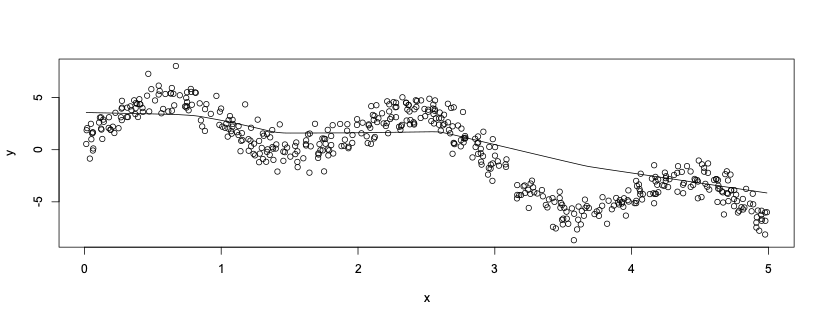
\includegraphics[width = \textwidth]{figs/nonLinWithNN.png}}
%     \only<3>{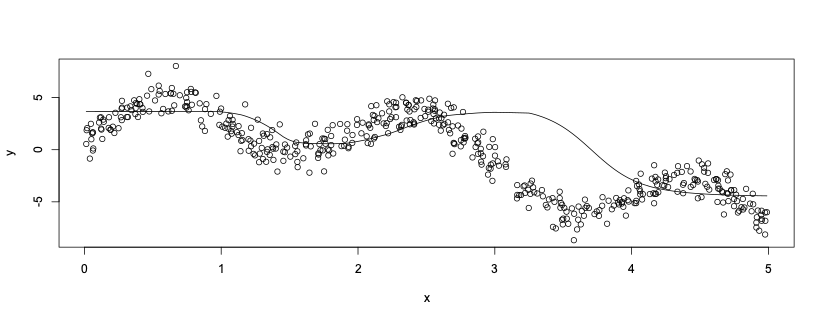
\includegraphics[width = \textwidth]{figs/nonLinWithNNtanh.png}}

% \end{frame}

\begin{frame}{Stegfunktion}

    Ett alternativ är att använda en steg-funktion, vi delar in $x$ i ett antal regioner $C_j$:
    \begin{equation*}
        y_i = \beta_1 \mathbb{I}(x_i \in C_1) + \beta_2 \mathbb{I}(x_i \in C_2) + \ldots + \beta_k \mathbb{I}(x_i \in C_k) + \varepsilon_i.
    \end{equation*}
    
    Vilka områden ska vi välja?

    \only<2>{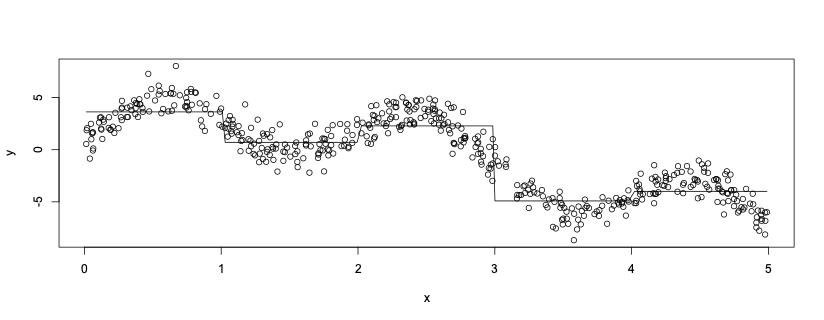
\includegraphics[width = \textwidth]{figs/nonLinWithSteps5.png}}
    \only<3>{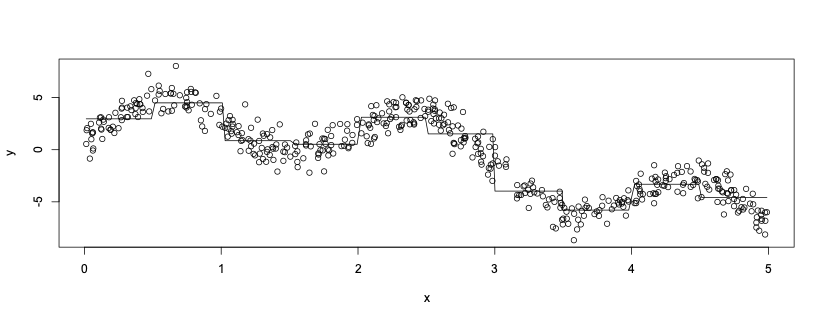
\includegraphics[width = \textwidth]{figs/nonLinWithSteps10.png}}

\end{frame}

\begin{frame}{Polynomregression och stegfunktioner}
    
    Fördelar:
    \begin{itemize}
        \item Generellt applicerbara.
        \item Enkelt att skala upp komplexiteten (fler polynom, fler områden).
    \end{itemize}

    Nackdelar:
    \begin{itemize}
        \item Svårt i högre dimensioner.
        \item Svårt att prediktera utanför data.
        \item Polynom av en hög ordning kan ofta vara "instabila"
        \item Stegfunktioner: hur många och vilka områden ska väljas?
    \end{itemize}
\end{frame}

\begin{frame}{Basfunktioner}
    Gemensamt för dessa metoder är att de bygger på basfunktioner.

    Givet ett gäng funktioner $(b_1(x), b_2(x), \ldots, b_k(x))$ kan vi göra regression som
    \begin{equation*}
        y_i = \beta_0 + \beta_1 b_1(x_i) + \beta_2 b_2(x_i) + \ldots + \beta_k b_k(x_i) + \varepsilon_i.
    \end{equation*}

    Observera att vi har ett linjärt problem (i basfunktionerna), vi kan enkelt skatta parametrarna $\beta$ som i vanlig linjär regression, dvs med OLS

\end{frame}

\begin{frame}{Basfunktioner}

    Basfunktioner kommer i många olika former:
    \begin{itemize}
        \item Polynom: $b_i(x) = x^i$.
        \item Stegfunktioner: $b_i(x) = \mathbb{I}(x \in C_i)$ där $C_i$ är något intervall.
        \item Andra funktioner är också vanliga, t.ex. $\log$, $\exp$, $\sin$, $\cos$, osv.
    \end{itemize}
    
    Ett problem: Behöver ofta väldigt många basfunktioner för att väl anpassa data. Leder ofta till överanpassning.

\end{frame}

\begin{frame}{Stegvisa basfunktioner}

    \begin{greenbox}
        Idé: Istället för att anpassa ett polynom (eller annan funktion) till hela datarymden. Anpassa en funktion per intervall.
    \end{greenbox}

    Modellen blir då:
    \begin{equation*}
        y_i = \begin{cases}
            h_0(x_i) + \varepsilon_i, & x_i \in C_0 \\
            \vdots & \vdots \\
            h_K(x_i) + \varepsilon_i, & x_i \in C_K,
        \end{cases}
    \end{equation*}
    där varje funktion $h_i$ ges av
    \begin{equation*}
        h_i(x) = \beta_{0,i} + \beta_{1,i} b_1(x) + \ldots + \beta_{k,i} b_k(x).
    \end{equation*}

    Vi löser helt enkelt en massa "simpla" problem på olika intervall.
    
\end{frame}

\begin{frame}{Stegvisa basfunktioner - Exempel}

    Vi delar upp data i fyra intervall. $x<1$, $1 \leq x < 2.5$, $ 2.5 \leq x < 4$ och $4 \leq x$ och skattar en kvadratisk funktion i varje intervall.

    \includegraphics<1>[width=\textwidth]{figs/nonLinGG.png}
    \includegraphics<2>[width=\textwidth]{figs/nonLinPieceQuad.png}
    %\includegraphics<3>[width=\textwidth]{figs/nonLinPieceQuadCont.png}
    
\end{frame}

\begin{frame}{Regression Splines}
    Stegvis polynomregression som i exemplet innan är en form av Regression Splines.

    \begin{bluebox}
    Målet är att anpassa en stegvis polynomfunktion med begränsningar i skarvarna för att få kontinuitet, kontinuerliga derivator osv.
    \end{bluebox}

    Termonologi:
    \begin{description}
        \item[knut (knot)]: Antal brytpunkter som vi använder oss av.
        \item[frihetsgrader (degrees of freedom)]: Antal parametrar som skattas.
        \item[trunkerad polynombas (truncated power basis)]: en funktion $h(x,\xi)$ som ges av
        \begin{equation*}
            h(x,\xi) = (x - \xi)^p_+ = \begin{cases}
                (x - \xi)^p & \text{if } x > \xi, \\
                0 & \text{otherwise.}
            \end{cases}
        \end{equation*} 
    \end{description}
\end{frame}

\begin{frame}{Regression splines}
    
    \begin{greenbox}
        Vårt mål: Skatta en stegvis polynomfunktion av grad-d under begränsningen att den ska vara kontinuerlig (kanske även kontinuerliga derivator).
    \end{greenbox}

    Ett grad-d polynom regression med $K$ knutar kan modelleras med basfunktioner som
    \begin{equation*}
        y_i = \beta_0 + \beta_1 b_1(x_i) + \beta_2 b_2(x_i) + \ldots + \beta_k b_k(x_i) + \varepsilon_i,
    \end{equation*}
    för ett lämpligt val av basfunktioner. Observera att $k \neq K$.

\end{frame}

\begin{frame}{Regression splines - Basfunktioner}

    För att få till ett grad-d polynom med rätt egenskaper skapar vi en modell som
    \begin{multline*}
        y_i = \beta_0 + \beta_1 x_i + \beta_2 x_i^2 + \ldots \beta_d x_i^d \\
        + \beta_{d+1} h(x_i, \xi_1) + \beta_{d+2} h(x_i, \xi_2) + \ldots + \beta_{d+K} h(x_i \xi_K) + \varepsilon_i,
    \end{multline*}
    där $h(x, \xi) = (x - \xi)^d$.

    Antal frihetsgrader:
    \begin{itemize}
        \item För ett grad-d polynom har vi $d+1$ frihetsgrader.
        \item Med $K$ knutar ($K+1$ intervall) får vi $(K+1)\cdot(d+1)$ frihetsgrader.
        \item Regression splines ger $d + 1 + K$ frihetsgrader.
    \end{itemize}
    
\end{frame}

\begin{frame}{Regression splines - Sammanfattning}

    \begin{itemize}
        \item Att dela upp och skatta oberoende polynom i varje intervall ger diskontinuerlig funktion.
        \item För varje begränsning (kontinuerlig, kontinuerliga derivator) minskar antalet frihetsgrader.
        \item Vilken grad ska vi välja?
        \begin{itemize}
            \item Vanligt med kubiska polynom (grad-3).
        \end{itemize}
        \item Hur välja antal knutar och deras placeringar?
        \item Skattningar utanför intervallet blir dåliga.
        \begin{description}
            \item[Natural spline]: Lägger till ett extra krav, att funktionen ska vara linjär i ändarna (innan första och efter sista knuten). 
        \end{description}
        \item Jämfört med vanlig polynomregression skulle vi behöva grad $d+k$ för samma antal frihetsgrader.
    \end{itemize}
    
\end{frame}

\begin{frame}{Natural Splines - Exempel}

    Vi modellerar med kubiska splines med knutar i $1,2,3$ och $4$.

    \uncover<2->{Lägger till Natural Splines med samma knutar.}

    \uncover<3->{Lägger till nya knutar i $0.5$ och $4.5$ och kör natural splines.}
    
    \includegraphics<1>[width=\textwidth]{figs/nonLinPeceBS.png}
    \includegraphics<2>[width=\textwidth]{figs/nonLinPeceBSNS.png}
    \includegraphics<3>[width=\textwidth]{figs/nonLinPeceBSNS2.png}

\end{frame}

\begin{frame}{Antal knutar och deras placeringar}
    
\begin{itemize}
    \item Funktionen kommer ha mest flexibilitet vid knutarna.
    \begin{itemize}
        \item Knutarna tillåter parametrarna att ändras.
        \item Placera fler knutar där du tror att det behövs.
    \end{itemize}
    \item Specificera antalet frihetsgrader och sprid ut knutarna jämnt.
    \begin{itemize}
        \item Givet en förbestämd grad $d$ så är antalet frihetsgrader $d+1+k$
        \item Fler frihetsgrader ger fler knutar.
    \end{itemize}
    \item Använd korsvalidering för att bestämma antalet.
\end{itemize}

\end{frame}

\begin{frame}{Antalet knutar och deras placeringar - Exempel}

    Vi använder samma data som tidigare och beräknar MSE för olika frihetsgrader

    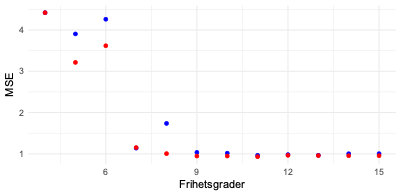
\includegraphics[width=\textwidth]{figs/bsnsMSE.png}
    

\end{frame}

\begin{frame}{Antalet knutar och deras placeringar - Exempel}

    Bästa modellen ser vi $8$ frihetsgrader för natural splines och $9$ frihetsgrader för cubic splines.

    Det ger 4 respektive 5 knutar.

    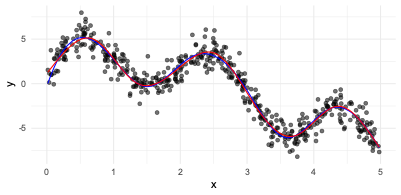
\includegraphics[width=\textwidth]{figs/bestMSE.png}
    

\end{frame}

\begin{frame}{Smoothing Splines}
    
    \begin{greenbox}
        Vårt mål är att hitta en funktion $g(x)$ som passar vår data väl.
    \end{greenbox}

    Ett generellt sätt att göra detta på är att hitta $g$ som minimerar
    \begin{equation*}
        \operatorname{RSS} = \sum_{i=1}^{n}(y_i - g(x_i))^2
    \end{equation*}

    Problem: Utan begränsningar på $g$ kan vi alltid få $\operatorname{RSS}$ till 0.

    Vad vi vill ha är en funktion som passar data bra men också är "mjuk".

\end{frame}

\begin{frame}{Mellanspel - Derivator}

    Givet en funktion $g(x)$, låt $g'(x)$ beteckna dess förstaderivata och $g''(x)$ dess andraderivata.

    \begin{itemize}
        \item Förstaderivatan $g'$ är lutningen (hastigheten) av en kurva.
        \item Andraderivatan $g''$ är hur lutningen ändrar sig (acceleration).
    \end{itemize}

    Vi kan se andraderivatan som ett mått på funktionens grovhet (roughness).

    Ett sätt att mäta grovhet av en funktion är att summera andraderivatan över funktionen (kontinuerlig funktion = integral)
    \begin{equation*}
        \int g''(x)^2 \mathrm{d}x.
    \end{equation*}

    Linjär funktion har $g''(x) = 0$ vilket är en helt mjuk funktion.

    Om $g(x)$ rör sig väldigt mycket kommer integralen bli väldigt stor.
\end{frame}

\begin{frame}{Smoothing Splines}

    Vi kan använda måttet för att skatta en funktion som har en viss "mjukhet".

    \begin{greenbox}
        Hitta funktionen $g(x)$ som minimerar
        \begin{equation*}
            L_{\text{Sm.Spl.}} = \sum_{i=1}^{n}(y_i - g(x_i))^2 + \lambda \int g''(x)^2 \mathrm{d}x \qquad \lambda \ge 0
        \end{equation*}
    \end{greenbox}
    
    Använder förlustfunktion + straffterm likt regularisering vi sett tidigare i Ridge och LASSO.

    \begin{itemize}
        \item Om $\lambda = 0$ har vi ingen begränsning.
        \item Om $\lambda = \infty$ får vi linjär funktion.
    \end{itemize}
\end{frame}

\begin{frame}{Smoothing splines}

    \begin{equation*}
        L_{\text{Sm.Spl.}} = \sum_{i=1}^{n}(y_i - g(x_i))^2 + \lambda \int g''(x)^2 \mathrm{d}x.
    \end{equation*}

    \begin{bluebox}\myheading{Teorem:}
        Funktionen $g(x)$ som optimerar förlustfunktionen är stegvis kubiskt med knutar i (unika) punkterna $(x_1, x_2, \ldots, x_n)$ och linjär utanför detta område.
    \end{bluebox}

    Resultatet är naturliga splines, men inte samma som om man gjort optimeringen som tidigare med samma knutar.

    Det blir en "krympt" version av dessa naturliga splines där krympningen beror på $\lambda$.
    
\end{frame}

\begin{frame}{Smoothing Splines - Sammanfattning}

    \begin{itemize}
        \item Efter optimering får vi kubisk natural splines.
        \item En knut i varje datapunkt.
        \item För många frihetsgrader? ($4+n$)
        \item $\lambda$ krymper parameterarna vilket ändrar den effektiva frihetsgraden $df_{\lambda}$.
        \begin{itemize}
            \item $\lambda = 0$ ger $df_{\lambda} = 4+n$.
            \item $\lambda = \infty$ ger $df_{\lambda} = 2$.
            \item Ofta vill vi istället välja $\lambda$ som ger oss viss frihetsgrad.
        \end{itemize}
        \item Hur välja $\lambda$?
    \end{itemize}
    
\end{frame}

\begin{frame}{Att välja $\lambda$}
    
    Eftersom smoothing splines resulterar i natural splines med ett fixt antal knutar med ridge regularisering kan vi skriva
    \begin{equation*}
        \hat{\mathbf{g}}_{\lambda} = \mathbf{S}_{\lambda} \mathbf{y},
    \end{equation*}
    där $\hat{\mathbf{g}}_{\lambda}$ är lösningen för vårt problem.

    Matrisen $\mathbf{S}_{\lambda}$ kallas utjämningsmatris (smoothing matrix).

    Se Kap 5.4 i \href{https://hastie.su.domains/ElemStatLearn/}{Elements of Statistical Learning} för tekniska detaljer.

\end{frame}

\begin{frame}{Effektiva frihetsgrader}

    En intressant detalj från formeln är att hur vi hittar $\hat{\mathbf{g}}_{\lambda}$ beror bara på data $x_i$ och $\lambda$ \imp{inte} på $\mathbf{y}$.

    Ett annat resultat är att vi kan definera effektiva frihetsgraderna som
    \begin{equation*}
        df_{\lambda} := \operatorname{tr}(\mathbf{S}_{\lambda}) = \sum_{i=1}^{n} \{\mathbf{S}_{\lambda}\}_{ii}.
    \end{equation*}

    Eftersom knutarna positioner är förbestämda $x_i$ så behöver vi bara bestämma $\lambda$.

\end{frame}

\begin{frame}{LOOCV}

    Det visar sig (igen see Elements of Statistical Learning för detaljer) att vi kan beräkna leave-one out cross-validation felet ($\text{RSS}_{\text{cv}}$) väldigt effektivt,
    \begin{equation*}
        \operatorname{RSS_{\text{cv}}} = \sum_{i=1}^{n}(y_i - \hat{g}_{\lambda}^{(-i)}(x_i))^2 = \sum_{i=1}^{n}\left[ \frac{y_i - \hat{g}_{\lambda}(x_i)}{1 - \{\mathbf{S}_{\lambda}\}_{ii}} \right]^2.
    \end{equation*}
    
    Observera: Vi behöver bara funktionen anpassad på all träningsdata för att beräkna detta.

\end{frame}

\begin{frame}{Smoothing Splines - Exempel}
    
    Använder samma data som tidigare.

    Skattar smoothing splines med effektiva frihetsgrader $9$. (Blå)

    Använder också LOOCV för att hitta bästa värdet $20.6$. (Röd)

    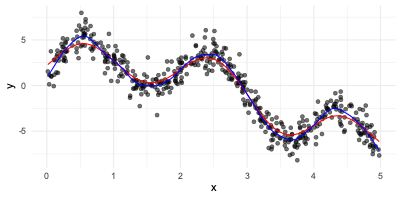
\includegraphics[width=\textwidth]{figs/bestCV.png}

\end{frame}



\begin{frame}{Smoothing Splines för klassificering}
    
    Vi har hittills gjort smoothing splines för regression, vi kan såklart använda metoden för klassificering.

    För logistisk regression har vi
    \begin{equation*}
        p(x) = \mathbb{P}(Y = 1 | X = x) = \frac{e^{f(x)}}{1 + e^{f(x)}},
    \end{equation*}
    där $f(x)$ är en linjär funktion.

    Vi kan såklart använda smoothing splines istället.

\end{frame}

\begin{frame}{Smoothing Splines för Klassificering}
    Om vi skriver upp optimeringsproblemet får vi log-likelihood (med straffterm)
    \begin{equation*}
        \ell = \sum_{i=1}^{n} \left[y_i f(x_i) - \log(1 + e^{f(x_i)}) \right] - \frac{1}{2}\lambda \int \{ f''(x)\}^2 \mathrm{d}x.
    \end{equation*}

    Vilket igen kan visas resultera i natural splines med knutar i datapunkterna.
\end{frame}

\begin{frame}{Flerdimensionella Splines}
    
    Hittills har vi pratat om endimensionella modeller. Alla går utöka till flerdimensionella modeller.

    Antag att vi har $x \in \mathbb{R}^2$ och att vi har basfunktioner $h_{1k}(x_1), k = 1, \ldots, K_1$ för första koordinaten $\qquad$ och motsvarande $h_{2k}(x_2), k = 1, \ldots, K_2$ för andra koordinaten.

    Vi kan då definera den $K_1 \times K_2$ dimensionella tensorprodukten basen
    \begin{equation*}
        g_{jk}(x) = h_{1j}(x_1)h_{2k}(x_2), j = 1,\ldots,K_1 \, k = 1, \ldots, K_2.
    \end{equation*}

    Dessa baser kan vi använda för att beskriva vår tvådimensionella funktion
    \begin{equation*}
        g(x) = \sum_{j=1}^{K_1} \sum_{k=1}^{K_2} g_{jk}(x).
    \end{equation*}

\end{frame}

\begin{frame}{Flerdimensionella Smoothing Splines}
    Vi kan igen sätta upp smoothing splines problemet för dessa flerdimensionella problem. Om $x_i \in \mathbb{R}^d$ ställer vi upp problemet
    \begin{equation*}
        \min_g \sum_{i=1}^{n}\{y_i - g(x_i)\}^2 + \lambda J[g],
    \end{equation*}
    där $J[g]$ är en lämplig straffterm.

    Om $d=2$ har vi
    \begin{equation*}
        J[g] = \int \int_{\mathbb{R}^2} \left[ \left( \frac{\partial^2 g(x)}{\partial x_1^2}\right)^2 + 2 \left(\frac{\partial^2 g(x)}{\partial x_1 \partial x_2}\right)^2 + \left(\frac{\partial^2 g(x)}{\partial x_2^2}\right)^2  \right] \mathrm{d}x_1 \mathrm{d} x_2
    \end{equation*}
\end{frame}

\begin{frame}{Flerdimensionella Smoothing Splines}

    Precis som för endimensionella smoothing splines har vi
    \begin{itemize}
        \item $\lambda = 0$ ger en funktion som interpolerar alla datapunkter.
        \item $\lambda = \infty$ ger ett plan.
        \item Andra värden ger en lösning som kan representeras som en linjärfunktion av basfunktioner med koefficient från ridge regression.
    \end{itemize}

    Lösningen är inte kubiska basfunktioner (som i endimensionella fallet) utan \imp{radiala basfunktioner} (radial basis functions).

    Också kallade \imp{thin-plate splines}.
    
\end{frame}

\end{document}